\chapter{}\label{chap5}
\addtocontents{toc}{\bigskip}
\addtocontents{toc}{\protect\contentsline{chapter}{\protect \centerline{Chapter \numberline{\thechapter}}}{}}  
\addtocontents{toc}{\medskip}

\heading{Lady Raman}
\addtocontents{toc}{\protect\contentsline{section}{Lady Raman}{\thepage}}
\vskip .25cm

\lhead[{\it\fontsize{9pt}{9pt}\selectfont\thepage}]{\it{\fontsize{9pt}{11pt}\selectfont Lady Raman}}

\index{Raman, Chandrasekhara Venkata!Raman, Lokasundari|(}

\noindent
A few remarks about Lokasundari Raman will not be out of place here. Those who have known her have often admired her devotion to her husband. On several journeys, she used to travel with him and look after him. Her principal interest in life was only one and that was to enable Professor Raman to carry on his scientific work in an uninterrupted manner. Seldom did she permit the projection in public of her own personality distinct from that of her husband's. This aspect of hers, besides being in accordance with the best of Indian traditions, was so noticeable on occasions that she drew the admiration of all concerned.

Lady Raman was of gentle nature. She moved around with grace and dignity, dressed always in simple sarees and with practically no jewellery. She spoke several languages; Tamil was her mother tongue, but she could speak Bengali fluently. She could also converse in English, Telugu, Kannada and Hindi. She was active in many social organisations devoted to the causes of women, children, the depressed and the poor.

There was a discussion (in the early part of 1936) between\break Mahatma Gandhi\index{Gandhi, Mahatma} and Lady Raman which reveals her nature and her interests. Gandhiji is reported to have told Lady Raman that he would be willing to visit the Institute of Science if Raman would be willing to show him some magic there! He also said to Lady Raman, ``I have heard all kinds of good things about you from your husband, but I have to find out how far they are true. He told me the other day that whilst he is absorbed in his Science, you find time for all kinds of humanitarian activities.''

Lady Raman replied, ``Not as much as I should be doing. But I am certainly interested in Khadi and Harijan welfare and social service and things of that kind. You know, Mahatmaji, I have been a spinner for many years. Some fifteen years ago I sent you a quantity of my own hand-spun yarn to be woven into cloth, and the late Madanlal Gandhi\index{Gandhi, Madanlal} sent the cloth on to me. But my husband had no faith in the wheel then. He would put away my wheel, smash it and break it; but I am glad to tell you that in my own lifetime the day has come when he no longer ridicules the wheel. He too believes in it''.

``Gandhi said,\index{Gandhi, Mahatma} ``I am very happy. Well, then, I want you to do a little work for me. Did you ever meet the late Kamala Nehru?''\index{Nehru, Kamala} Lady Raman replied, ``Once or twice, Mahatmaji. But I know the old Mrs. Nehru very well''. Gandhi said, ``But you, of course, know what a good woman Kamala was. You know how she spent herself for the country. But when I prize most of her is not her political contribution, but her great spiritual beauty which I should like every man and woman to know.''

Lady Raman butted in, ``Yes, I know of her services and her moral beauty''.

To which Gandhiji said, ``Then you must help me in collecting some money for the Memorial we are having for her''.

Lady Raman heartily agreed. As this dialogue was going on, in came Sir C.V. Raman. She was talking in Hindi as he came in. ``Now, is that Hindi any good?'' he asked jocularly, to which Gandhiji replied, ``Certainly as good as your Science''. 

``Oh, yes,'' said Raman. ``She has an amazing capacity for picking up languages. She knows Hindi, she knows Bengali better than Hindi.''

Gandhiji put in, ``Of course, she has stayed in Calcutta for some years''.

\eject

Raman replied, ``Not necessarily for that reason. I, too, have stayed with her. But I know not a word. And now, here, she has picked up Kannada and talks it''. Raman then began wondering what language could be the language for the masses of India and seemed for a moment to incline towards English ({\em Harijan}, 6.6.36).

Lady Raman's main interest was to take care of Raman; serving him with food at the proper time and compelling him to take sufficient rest. She managed her home very efficiently and always put her interests after her duty towards her husband. There was a person to take care of the kitchen, but Lady Raman was good at cooking and could very well manage by herself when the occasion demanded. She always had other persons in the house as well; often relatives and, quite frequently, someone, especially women, who needed help and shelter. She had a compassionate heart and took upon herself the task of helping the poor and the helpless.

Lady Raman was a self-educated person. By association with Raman and his vast coterie of admirers and students, she picked up a phenomenal amount of knowledge about various things. She could deal with almost any situation. Her account of Raman's trip to Stockholm to receive the Nobel Prize is replete with humour, fine details and marvellous descriptions. Raman often delegated to her the care of routine matters connected with the Institute. When it came to worldly matters, she was Raman's trusted adviser.

Once, she planned to take some visitors round the museum of the Raman Institute.\index{Raman Research Institute} I volunteered to accompany them and explain to the visitors the various scientific aspects of the exhibits, but she did not accept my offer and told me that she could manage by herself. However, I did accompany the party and found myself a silent spectator listening to Lady Raman doing an excellent job as she explained the nature of crystals, in particular the nature of diamond, in very simple language. The visitors, were quite impressed with her commentary.

Raman's total absorption in Science must have been hard on her, for in later years, she turned somewhat cynical in her attitude. She could be absolutely charming, very helpful and very warm. But at other times her attitude would be different. Lady Raman loved her two sons very much, but the older son, Chandrasekhar,\index{Chandrasekhar, V.} had left the house, for his lifestyle and ideas were not consistent with Raman's. The second son, Radhakrishnan,\index{Radhakrishnan, V.} also left India a few years after graduating in Physics from Mysore University,\index{Mysore University} and spent a long time abroad before he returned to accept the Directorship of the Raman Research Institute. All these happenings turned Lady Raman somewhat bitter, but her devotion to Raman was in no way affected.

At the time of Raman's death, when his body was being removed from the Hall, she stood by and wept like a child. She said, ``I took care of him for more than sixty years and you are all taking him away from which he will never return''. It was heart-rending to see the grand old lady break down like this. She was, of course, a very strong person with a strong will, and recovered from the shock. When Radhakrishnan returned to Bangalore to assume the Directorship, she felt very happy and became her old self. During my visits to India between 1971 and 1980 I always called on her and she was very cordial. Lady Raman lived for ten years after Raman's death and passed away in May 1980. It was a great satisfaction to her to see her grandson born and Radhakrishnan firmly established in Bangalore as the head of the Raman Research Institute.
\index{Raman, Chandrasekhara Venkata!Raman, Lokasundari|)}
\begin{figure}[H]
\centering
\includegraphics[scale=.92]{eps/17.eps}

{\fontsize{10pt}{12pt}\selectfont \em Kausalya Ramaseshan, Lokasundari Raman, Kamala Jayaraman}\relax
\end{figure}

\begin{figure}[H]
\centering
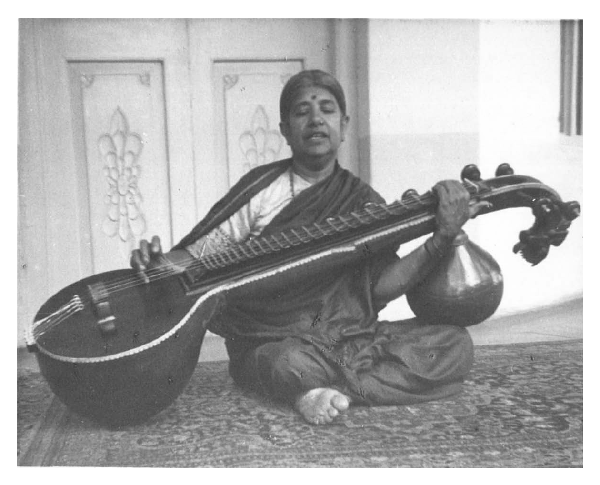
\includegraphics[scale=.95]{eps/16.eps}

{\fontsize{10pt}{12pt}\selectfont\em Lady Raman playing Veena}\relax

{\fontsize{10pt}{12pt}\selectfont (Photo Credit: Dominique Radhakrishnan)}\relax
\end{figure}

\heading{V. Radhakrishnan}
\addtocontents{toc}{\protect\contentsline{section}{V. Radhakrishnan}{\thepage}}
\vskip .12cm

\lhead[{\it\fontsize{9pt}{9pt}\selectfont\thepage}]{\it{\fontsize{9pt}{11pt}\selectfont V. Radhakrishnan}}

\index{Radhakrishnan, V.|(}

\noindent
Radhakrishnan, the second son of the Ramans was known to his friends simply as Rad. He was born on May 19, 1929, just after Raman discovered his Effect. My first contact with him was in November 1949, soon after I joined the RRI in Bangalore. In the large compound of `Panchavati', Raman's residence in Malleswaram, Rad occupied a nice little cottage in the northwest corner, connected to the main bungalow and the kitchen-dining complex by a covered corridor. 

Rad was very interested in electronics and had a lot of books and journals in the cottage, all neatly arranged, as well as a complete set of the magazine `Amateur Radio'. He was still a student at the Central College in Bangalore doing his B.Sc. (Hons.) course in physics when I first met him. Rad was very friendly to me and we used to meet frequently. I learnt a lot of electronics from him, for I was myself an amateur electronics enthusiast. Further, he introduced me to astronomy and took me out to identify stars and constellations. In due course we got to know each other very well. After he finished his studies at the Central College he joined the I.I.Sc.\@ Physics Department that was headed by Prof R.S. Krishnan at the time.

However, he didn't stay there long. Around 1953, Prof.\@ Rydbeck (from the Chalmers Institute of Technology, Sweden) who was doing important work in radio astronomy visited Bangalore. I remember his visit to our Institute very well, and he gave an excellent talk. Radhakrishnan and Rydbeck got to know each other well and out of that visit Radhakrishnan must have made up his mind to pursue radio astronomy. I think Rydbeck extended Rad an invitation to join his group, and one fine day Rad left Bangalore and went off to England. For a couple of years I lost touch with him. I don't know when exactly he joined Rydbeck's group, but I heard that he had done some outstanding work concerning radio emissions from Jupiter, a very significant contribution. 

Soon after I joined UCLA, my friend Venkateswaran in the  Meteorology department told me that Rad was in Caltech and living in Pasadena. I got in touch with him and he was very cordial. He came to see me and took me to his apartment to spend a weekend. Over several south Indian meals that I managed to cook in his apartment with improvised ingredients -- Rad loved Indian food -- we caught up on things. During another visit he took me to the radio telescope facilities at Owens Valley and I spent two days with him when he showed me the huge dishes and how they collect data. I think he worked in the group headed by John Bolton, a well-known radio astronomer from Australia at the Caltech facility. I was fascinated by what all I saw. Rad also drove me to the neighboring San Gabriel mountains and for first time in my life I saw so much snow! We threw snowballs at each other and played like children. He also took me around Caltech and pointed out some of the famous people of those times. After my wife Kamala arrived in Los Angeles we used to invite Rad to our home on Levering Avenue in Westwood. He was fond of my daughters, and he also loved all the food that Kamala prepared. We always conversed in Tamil.

\eject

He then moved to New Jersey, to Bell Labs, to learn about microwave amplifiers. Derrick Scovil was an expert in the field, and Bell Labs had decided to help the Caltech group by building a microwave amplifier, then a very sophisticated device. I think Rad spent something like a year in Derrick's group and learnt all about operating the amplifier which he incorporated in the Owens Valley facility. During his Bell Labs days I visited him, and he helped me meet some people there.  I was fascinated with the laser programme, as well as the large number of renowned scientists I had heard of. Again, our stay in his apartment gave us time to talk about my research in UCLA. 

\vskip .1cm

There was a break of 7 or 8 years before we met again. I knew that he went to Australia after Caltech and became very well-known in the field of radio astronomy. In the meantime he got married to Dominique and came to the US with her -- it must have been 1968 or 1969. They visited us at Murray Hill and were our guests for a few days. We enjoyed their visit very much except that Rad smoked a lot and I did not have the heart to tell him not to.

\vskip .1cm

We then met in Bangalore in 1970, soon after the passing away of his father. I was spending a sabbatical year there at that time, setting up facilities for high-pressure research in India. Rad talked to me about the pressure being applied to him to accept the responsibility of running the Raman Institute. I told him he could do a lot of good for Indian science by accepting the challenge. He finally made the decision to move to Bangalore as Director of the RRI, and it flourished under his leadership for over two decades. Rad encouraged good research and set high standards for it, and his own scientific stature rose to new heights both in India and internationally.

\vskip .1cm

Rad's interests were very varied. He built flying machines and boats to sail long distances in hostile oceans! During one of our visits he showed me the flying machine and talked lightly about the near fatal accident he had and survived. He showed me the features of the ``Catamaran'' sail boat that he was building, and its modern navigation guidance systems. I was told that he did take it out to Cochin and sailed in the Indian Ocean but things did not go well because of a storm and he had to abandon the trip.


The last time I saw him was in December 2009. He took me to his home and we had lunch prepared by Dominique. Earlier in his office we talked and at one point I became emotional when discussing Professor Raman, and his words were comforting. I learned with great sorrow that he passed away in Bangalore on March 3, 2011. I wrote a note to Dominique and she graciously responded despite her deep sorrow. She continues to live in Bangalore in the same house, perpe\-tuating the memory of her great husband, just like Lady Raman did.

Rad was a chip of the old block in many ways. Fiercely independent, he treated people with due respect no matter where in the ladder they belonged. He listened to grievances of all Institute employees and was very fair in his dealings. So I have heard, and knowing his personality, I believe it to be true. He appreciated gifted individuals no matter whether they had degrees or not. He himself set an example by not going for any degrees.


Rad earned his status by outstanding accomplishments in his field. It was a privilege to have known him.
\index{Radhakrishnan, V.|)}
\begin{figure}[H]
\centering
\includegraphics{eps/18.eps}

{\fontsize{10pt}{12pt}\selectfont\em V. Radhakrishnan.}\relax
\end{figure}

\begin{figure}[H]%check width of image
\centering
\includegraphics[scale=.8]{eps/19.eps}

{\fontsize{10pt}{12pt}\selectfont\em Rad with his family.}\relax
\end{figure}

\begin{figure}[H]
\centering
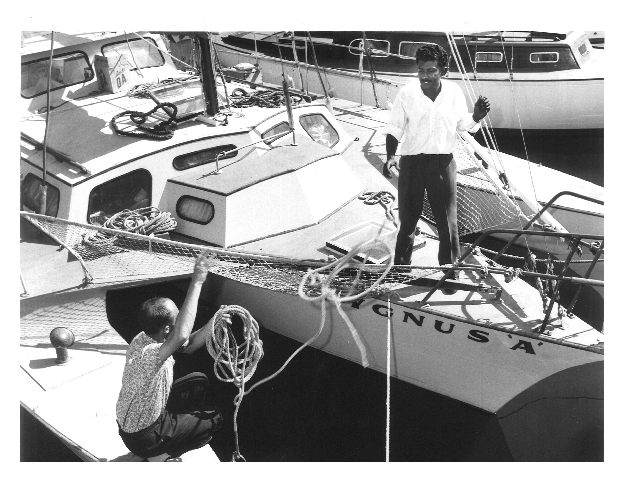
\includegraphics[scale=.95]{eps/20.eps}

{\fontsize{10pt}{12pt}\selectfont\em Dave and Rad tying up in Sydney in 1966..}\relax
\end{figure}

\begin{figure}[H]
\centering
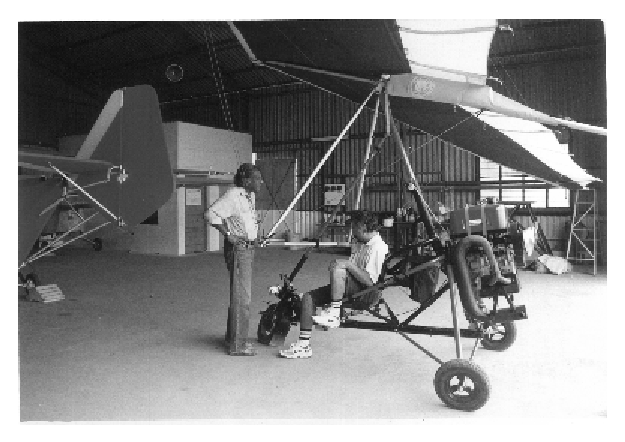
\includegraphics[scale=.95]{eps/21.eps}

{\fontsize{10pt}{12pt}\selectfont\em Rad with his hand-glider.}\relax

{\fontsize{10pt}{12pt}\selectfont (Photo Credit : Pages 213-214: Dominique Radhakrishnan)}\relax
\end{figure}

\heading{Raman's interest in music and musical instruments}
\addtocontents{toc}{\protect\contentsline{section}{Raman's interest in music and musical instruments}{\thepage}}
\vskip .1cm

\index{Raman, Chandrasekhara Venkata!Traits/Interests|(}

\lhead[{\it\fontsize{9pt}{9pt}\selectfont\thepage}]{\it{\fontsize{9pt}{11pt}\selectfont Raman's interest in music and musical instruments}}

\noindent
The scientific work of both Helmholtz\index{Helmholtz, Hermann Von} and Lord Rayleigh\index{Rayleigh, Lord} profoundly influenced Raman's thinking and research. In fact, Raman regarded Lord Rayleigh as his teacher in a very real sense, although he had never met him. Both these stalwarts had written marvellous treatises on sound. These books, which Raman had read in his student days, inspired him and, in the early days at the Indian Association for Cultivation of Science,\index{The Indian Association for Cultivation of Science} Raman took to research in acoustics. One of the aspects of sound he became deeply interested in was Indian musical instruments.

Music and mathematics have much in common, being essentially creations of the human mind. However, neither the mathematician nor the musician has generally cared to understand the world of the other. It was Pythagoras who felt at home in both spheres and was able to formulate what made a sound seem musical to the human ear. He discovered that the musical pitch of a vibrating string increased by an octave when its length was reduced by half, and from this developed his theory of harmony. If the string of an instrument was plucked, it not only emitted a note having a fundamental frequency, but also produced higher notes. The effect was musical if these overtones were in the ratios of 1:2:3 etc. These harmonic contents were the ones that makes the note sound pleasing to the ear.

Raman began his first serious work in acoustics working on the theory of bowed string-instruments. The vibrations of stretched str\-ings fascinated mathematicians and physicists alike, not only for the wealth of the mathematical problems they
provided, but also for the harmony of their tones. When Raman began his studies, the linear theory of vibrations of ideal strings was well developed, but, despite the existence of such celebrated violins as those of Stradivarius, there was little that could be asserted with adequate proof of how the vibrations of the strings of a musical instrument were governed or excited. In the course of his work on violins, Raman made fundamental contributions to the motion of the bowed point and the effect of the bridge in coupling the motion of the string to the body of the violin.

\eject

The work of Raman on the drums of India is epoch-making. The drum is amongst the oldest of musical instruments. Drums are to be found in almost all parts of the world in some form or other. The {\em tabla} and {\em mridangam}, two of the better-known percussion instruments of India, are of unknown origin and antiquity. They are unique among all drums, being the only ones that produced harmonic overtones, for the percussion group of instruments as a class can only produce anharmonic overtones and are, therefore, in a sense, only noise-makers. Raman perceived the musical sounds that emanate from Indian percussion instruments, and this excited him sufficiently to investigate the physics aspect of it. He showed that both the {\em tabla} and {\em mridangam} produced harmonic overtones and that this was achieved by the partial loading of the drum membrane with a firmly adherent but flexible paste. The harmonic overtones turned out to be the different modes of vibrations of a stretched but loaded membrane, which could be heard when appropriately excited. Raman was able to excite all these overtone modes by tapping the drum at the antinodes and restraining the motion of the drumhead by gentle constraints applied at suitable points with his fingertips. When he first discovered the harmonic character of these drums, there were no electronic oscillators or analysers; he had only his keen ear to rely on. Raman demonstrated the existence of these overtone modes by dusting the membrane with lycopodium powder and observing the pattern it produced on the excited membrane.

Decades later, the work on drums was taken up by Professor B.S. Ramakrishna\index{Ramakrishna, B.S.} at the Indian Institute of Science.\index{Indian Institute of Science@\textit{Indian Journal of Physics}} Investigating with sophisticated instruments and methods of excitation, Ramakrishna and his coworkers confirmed all Raman's earlier observations and conclusions. They have, since then, presented a comprehensive treatment of the subject.

The {\em veena} and the {\em tampura} are the oldest musical instruments of India and are revered as gifts of the Gods. Their tonal quality is perhaps the most pleasing to the ear. Raman made the discovery that certain overtones which, according to acoustical principles, should be entirely absent, came out with great intensity in these instruments. He showed that this violation of what is called the Young-Helmholtz law is due to the curved bridge which the ancient Hindus had discovered by experimenting and listening. The {\em veena} and {\em tampura} could produce sounds richer in quality. The latter in particular is indispensable for Indian instrumental and vocal music, setting the reference for the artist; it is known as the background drone.

Raman's acoustical studies were not confined to Indian musical instruments alone; they extended to Western ones as well. We have already mentioned his work on the violin. His mathematical theory of how the impact of the hammer produces the exquisite vibrations in a pianoforte, and his demonstration of the peculiar Wolf note produced by the violin and cello were all classics, accepted and recognised by experts the world over. In recognition of his outstanding contributions in this field, he was invited to contribute to those famous volumes, {\em Handbuch der Physik}.\index{Handbuch der Physik@\textit{Handbuch der Physik}} In the Sixties, the Catgut Acoustical Society\index{Catgut Acoustical Society} in America, a society devoted exclusively to the acoustics of violins, made him an honorary member.

Raman's interest in music was confined not merely to the strictly scientific aspects. He was familiar with South Indian classical music and had learnt to play the violin. Lady Raman\index{Raman, Chandrasekhara Venkata!Raman, Lokasundari} was an accomplished {\em veena} player and was very interested in Carnatic Music. I often saw her at musical concerts in Bangalore and went to a few with her. However, I never saw Raman at any concerts. Once, we were driving through a part of Bangalore where the famous South Indian classical vocalist M.S. Subbulakshmi\index{Subbulakshmi, M.S.} was singing at a wedding. Raman asked the driver to stop the car near the {\em pandal} so that we could hear her through the loud-speakers installed outside. We listened for about fifteen minutes and then Raman asked the driver to move on. He said to me, ``I say, Subbulakshmi's voice has changed now. Did you notice it?'' I replied that it was so and that she had now become a full-fledged Carnatic vocalist; both her voice and style of singing were very different from when she sang film music.

In the late Sixties, Raman would occasionally arrange for a violinist, Thathachar, to come to his house and play for him. Lady Raman apparently arranged this at his request.

Raman's elder brother, C. Subrahmanya Ayyar, was a noted musicologist who could play the violin expertly. He had also written a book called {\em Grammar of South Indian Carnatic Music}\index{Grammar of South Indian Carnatic Music@\textit{Grammar of South Indian Carnatic Music}} in which he analysed the South Indian {\em raga} system, in terms of the notes and their frequency relationships which make up the melodic scale. This is an excellent monograph on the theory of Carnatic Music. C.S. Ayyar, as he was known, was an active participant in the technical sessions of the Madras Music Academy.\index{Madras Music Academy} The Academy holds its annual session during the last two weeks in December every year and the finer points of classical music are discussed by experts.

A strong interest in music ran in the family and it is no surprise that Raman became so engrossed in the acoustics of musical instruments and made such monumental contributions in this field.
\index{Raman, Chandrasekhara Venkata!Traits/Interests|)}

\bigskip
\heading{The Raman Effect}
\addtocontents{toc}{\protect\contentsline{section}{The Raman Effect}{\thepage}}
\smallskip

\index{Raman, Chandrasekhara Venkata!Raman Effect}

\lhead[{\it\fontsize{9pt}{9pt}\selectfont\thepage}]{\it{\fontsize{9pt}{11pt}\selectfont The Raman Effect}}

\noindent
To explain what the Raman Effect is to a layman is not easy. It is necessary to be an advanced student of Science to comprehend it. However, the lecture Raman gave announcing his discovery, under the title ``A New Radiation'', is a masterpiece of exposition, set as it is in as simple a language as possible. This is a very important lecture historically and I am therefore reproducing it here for the benefit of readers.

There was also once a group of high school students from Tamil Nadu who came to visit the Raman Institute.\index{Raman Research Institute} There must have been 30 of them, led by two teachers. Raman took them round and, in explaining the crystals to them, he often broke into Tamil. The teachers who accompanied the group requested Professor Raman to explain to the students in Tamil what the Raman Effect was. Raman seated them in the lecture hall and explained to them in Tamil the nature of the Raman Effect. I was listening to the account he gave, for I was curious how he would go about it. The gist of what he said in Tamil would translate something like this.
\begin{quote}
{\fontsize{10pt}{12pt}\selectfont
``Think of a person throwing a tennis ball at a certain speed to a tennis player who is waving his bat back and forth. If the bat is moving backward when the ball hits the bat, the ball will lose some of its speed and bounce back with a reduced speed. Similarly, when the ball hits the bat while the bat is moving forward, the ball will gain speed from the forward moving bat and bounce back at a higher speed than the thrower put in.

The Raman Effect\index{Raman, Chandrasekhara Venkata!Raman Effect} has to do with light and molecules. You should think of the incoming light as the tennis ball thrown and the molecule as the tennis player who is moving his bat back and forth. The atoms in a molecule are vibrating constantly about the equilibrium position. Light also vibrates at a certain frequency (when it is monochromatic), and when it hits a molecule the frequency of the light is decreased or increased, depending upon the energy state of the molecule; the frequency of the light is increased when the molecule gives energy to the light, or decreased when the molecule takes energy from the light, like the ball gaining or losing its speed, as I've already stated.''}\relax
\end{quote}

Whether the students understood this analogy or not, it was a most apt way of putting it.

\bigskip
\heading{A new radiation\footnote{Inaugural Address delivered to the South Indian Science Association on Friday, March 16, 1928, at Bangalore, and published in the {\em Indian Journal of Physics}, 1928, Volume 2, pp. 387-398.}}
\addtocontents{toc}{\protect\contentsline{section}{A new radiation}{\thepage}}

\index{Raman, Chandrasekhara Venkata!Papers/Publications/Addresses}

\lhead[{\it\fontsize{9pt}{9pt}\selectfont\thepage}]{\it{\fontsize{9pt}{11pt}\selectfont A new radiation}}

\smallskip
\noindent
{\em Introductory}

\smallskip
I propose this evening to speak to you on a new kind of radiation or light-emission from atoms and molecules. To make the significance of the discovery clear, I propose to place before you the history of the investigations made at Calcutta which led up to it. Before doing so, however, a few preliminary remarks regarding radiation from atoms and molecules will not be out of place.

Various ways are known to the physicist by which atoms or mole\-cules may be caused to emit light, as, for instance, heating a substance or bombarding it with a stream of electrons. A light thus emitted is usually characteristic of the atoms or molecules and is referred to as {\em primary} radiation. It is also possible to induce radiation from atoms and molecules by illuminating them strongly. Such light-emission is referred to as {\em secondary} radiation. The familiar diffusion of light by rough surfaces may be cited as an example of secondary radiation, but, strictly speaking, it hardly deserves the name, being an effect occurring at the boundaries between media of different refractive indices and not a true volume-effect in which all the atoms and molecules of the substance take part. The first case discovered of secondary radiation really worthy of the name was the phenomenon of fluorescence whose laws were elucidated by the investigations of Sir George Stokes.\index{Stokes, George} This is a familiar effect which is exhibited in a very conspicuous manner in the visible region of the spectrum by various organic dye-stuffs. I have here a bottle of water in which an extremely small quantity of fluorescein is dissolved. You notice that when placed in the beam of light from the lantern, it shines with a vivid green light, and that the colour of the emission is not altered, though its brightness is changed by placing filters of various colours between the bottle and the lantern. A violet filter excites the green flourescence strongly, while a red filter has but little effect.

Another kind of secondary radiation whose existence has been experimentally recognised more recently is the scattering of light by atoms and molecules. It is this scattering that gives us the light of the sky, the blue colour of the deep sea and the delicate opalescence of large masses of clear ice. I have here a large bottle of a very clear and transparent liquid, toluene, which, as you notice, contains hardly any dust-particles, but the track of the beam from the lantern passing through it is visible as a brilliant blue cone of light. This internal opalescence continues to be visible even after the most careful purification of the liquid by repeated distillation {\em in vacuo}. A similar opalescence is shown, though much less brightly, by dust-free gases and vapours, and also by solids. A large clear block of ice shows a blue colour in the track of the beam when sunlight passes through it. The blue opalescence of blocks of clear optical glass is also readily demonstrable. The molecular scattering of light is thus a phenomenon common to all states of matter.

\eject

During the past seven years, the scattering of light in transparent media has been the subject of intensive experimental and theoretical investigation at Calcutta, and it is the researches made on this subject that have led to the discovery which I shall lay before you this evening. One important outcome of our researches has been to show that while light-scattering is in one sense a molecular phenomenon, in another sense it is a bulk-effect having a thermal origin. It is the thermal agitation of the molecules which causes them to be distributed and orientated in space with
incomplete regularity, and it is the local fluctuations in the properties of the medium thus arising which give rise to optical heterogenity and consequent diffusion of light. The subject of light-scattering is thus a meeting ground for thermodynamics, molecular physics and the wave-theory of radiation. That the combination of theories in such diverse fields of physics gives us predictions, which have been experimentally verified, is one of the triumphs of modern physics.

\medskip
\noindent
{\em A new phenomenon}
\smallskip

While the quantitative investigations made at Calcutta have in the main substantiated the thermodynamic-wave-optical theory of light-scattering, indications appeared even in our earliest studies of a new phenomenon which refused to fit in with our pre-conceived notions. Thus, in some observations made by me with the assistance of Mr. Seshagiri Rao\index{Rao, Seshagiri} in December 1921, it was found that the depolarisation of the light transversely scattered by distilled water measured with a double-image prism and Nicol increased very markedly when a violet filter was placed in the path of the incident-light. More careful investigations, made with dust-free liquids in 1922, confirmed this effect and showed it to exist also in methyl and ethyl alcohols, and, to a lesser degree, in ether. It was also noticed that the colours of the scattered light from the different liquids studied did not match perfectly.

\vskip .1cm

An important advance was made when Dr. Ramanathan, working at Calcutta in the summer of 1923, investigated the phenomenon more closely and discovered that it was not a true dependence of the depolarisation on the wavelength of the scattering radiation but was due to the presence in the scattered light of what he described as ``a trace of fluorescence''. This was shown by the fact that the measured depolarisation depended on whether the blue filter used was placed in the path of the incident-beam or of the scattered light, being smaller in the latter case. Accepting the explanation of the effect as ``weak fluorescence'', it naturally became important to discover whether it was due to some impurity present in the substance. Dr. Ramanathan tested this by careful chemical purification, followed by repeated slow distillation of the liquid at the temperature of melting ice. He found that the effect persisted undiminished.

\vskip .1cm

The investigation of this species of `weak fluorescence' has, ever since 1923, been on our programme of research at Calcutta. Krishnan, who investigated 60 liquids for light-scattering in the spring and summer of 1924, made systematic studies of the phenomenon, and found that it was shown markedly by water, ether, all the monohydric alcohols and a few other compounds. He pointed out that the liquids which exhibit the effect have certain family relationships amongst themselves, and that they are also substances whose molecules are known to be polar. The chemical importance of the subject led to Mr. S. Venkateswaran\index{Venkateswaran, S.} attempting to make a fuller study of it in the summer of 1925, but without any special success. The research was discontinued at the time but was resumed by him later in the current year (January 1928). The remarkable observation was made that the visible radiation which is excited in pure dry glycerine by ultraviolet radiation (sunlight filtered through Corning glass G. 586) is {\em strongly polarised}.

\vskip .1cm

The possibility of a similar effect in gases and vapours was also borne mind and repeatedly looked for by the workers at Calcutta. The feebleness of the scattering in gases and vapours, and the infructuousness of the earlier efforts in this direction, however discouraged progress.

\newpage

\noindent
{\em Its universality}
\smallskip

Though the phenomenon was described in the paper of Dr. Ramanathan and Mr. Krishnan as a ``feeble fluorescence'', the impression left on my mind at the time was that we had here an entirely new type of secondary radiation distinct from what is usually described as fluorescence. The publication of the idea was however discouraged by the belief then entertained that only a few liquids exhibited the effect and by the supposition that it was unpolarised in the same way as ordinary fluorescence in liquids. Indeed, a chemical critic might even have asserted that the effect was in each case due to a trace of dissolved fluorescent impurity present in the substance which our efforts at purification had failed to remove.

\vskip .1cm

Early this year, however, a powerful impetus to further research was provided when I conceived the idea that the effect was some kind of optical analogue to the type of X-ray-scattering discovered by Prof. Compton,\index{Compton, A.H.} for which he recently received the Nobel Prize in Physics. I immediately undertook an experimental re-examination of the subject in collaboration with Mr. K.S. Krishnan\index{Krishnan, K.S.} and this has proved very fruitful in results. The first step taken in the research was to find whether the effect is shown by all liquids. The method of investigation was to use a powerful beam of sunlight from a heliostat concentrated by a $7''$ telescope objective combined with a short focus lens. This was passed through a blue-violet filter and then through the liquid under examination contained in an evacuated bulb and purified by repeated distillation {\em in vacuo}. A second filter of green glass was used which was complementary in colour to the blue-violet filter. If it were placed in the track of the incident-light, all illumination disappears, while, if it be placed between the bulk and the observer's eye, the opalescent track within the liquid continued to be visible, though less brightly.

\vskip .1cm

All the liquids examined (and they were some 80 in number) showed the effect in a striking manner. There was therefore no longer any doubt that the phenomenon was universal in character; with the bulb of toluene on the lantern, you see that the effect is \hbox{readily} demonstrable. The cone of light vanishes when I place the violet and green filters together, but it appears when I transfer the latter to a place between my audience and the observation bulb.

Now the test with the complementary filters is precisely that ordinarily used for detecting fluorescence and indeed was first suggested by Stokes in his investigations on the subject. You may therefore rightly ask me the question how does this phenomenon differ from fluorescence? The answer to the question is, firstly, that it is of an entirely different order of intensity. A more satisfactory proof was however forthcoming when Mr. Krishnan and myself examined the polarisation of this new type of radiation and found that it was nearly as strong as that of the ordinary light-scattering in many cases, and is thus quite distinct from ordinary fluorescence which is usually unpolarised.

This is shown for the case of toluene in Figs. 1\label{pageref-1} and 2 in Plate XII. Fig. 1 is a photograph of the scattering by toluene of sunlight filtered through a blue-violet glass. It was taken through a double-image prism of iceland spar with an exposure of 3 seconds. Fig. 2 is a picture with an additional complementary filter of green glass interposed in front of the camera lens. The exposure necessary is now increased greatly by the insensitiveness of the plate to green light, and had to be as much as 25 minutes. It will be noticed that the polarisation of the track as shown by the difference in brightness of the two polarised images is quite as prominent in Fig. 2 as in Fig. 1.

I may also mention that Mr. Krishnan\index{Krishnan, K.S.} and myself have succeeded in detecting the new radiation and observing its partial polarisation in a number of organic vapours and also in the gases CO$_{2}$ and N$_{2}$O. The problem in these cases is one of securing sufficient intensity of scattering for the effect to be detectable through the complementary filter. This can be secured by heating up the substance in a sealed bulb or by using steel observation-vessels for containing the compressed gases, so as to obtain sufficient density of the scattering molecules. The question of the background against which the track is observed is also of great importance.

\eject

The new type of secondary radiation is also observable in crystals such as ice, and in amorphous solids. It is thus a phenomenon whose universal nature has to be recognised.

\medskip
\noindent
{\em Line-spectrum of new radiation}\label{pageref-2}
\smallskip

That the secondary radiation passes the complementary filter and yet is strongly polarised to an extent comparable with the ordinary molecular scattering, is clear evidence that we have in it an entirely new type of secondary radiation which is distinct from either the ordinary scattering or the usual type of fluorescence. A striking and even startling confirmation of this view is furnished by an examination of its spectrum. Preliminary observations, with sunlight filtered through a combination which passes a narrow range of wavelengths, showed the spectrum of the new radiation to consist mainly of a narrow range of wavelengths clearly separated from the incident spectrum by a dark space. This encouraged me to take up observations with a monochromatic source of light.

A quartz mercury lamp with a filter which completely cuts out all the visible lines of longer wavelength than the indigo line \hbox{4,358A.U}. was found to be very effective. When the light from such a lamp was passed through the bulb containing a dust-free liquid, and the spectrum of the scattered light was observed through a direct-vision spectroscope, it was found to exhibit two or more sharp bright lines in the blue and green regions of the spectrum. These lines are not present in the spectrum of the incident-light or in the unfiltered light of the mercury arc and are thus manufactured by the molecules of the liquid.

Figures 3(1) and 3(2), and Figs. 4(1) and 4(2) show the phenomenon. They are spectrograms taken with a small Hilger quartz instrument of the scattering by {\em liquid} benzene. Fig. 3 was taken with the light from the quartz mercury arc filtered through a blue glass which allows the wavelengths from about 3,500A.U. to 4,400A.U. to pass through. Fig. 3(1) represents the incident-spectrum and Fig. 3(2) the scattered-spectrum. and the latter shows a number of sharp lines not present in Fig. 3(1). These are indicated in the figure. Figs. 4(1) and (2) similarly represent the incident and scattered spectra with benzene liquid, the filter used being a potassium permanganate solution. Here again the new lines which appear are indicated in the figure. Visual observations were also made using a quinine sulphate solution together with the blue glass as a filter and thus cutting off all the radiations except 4,358A.U. from the incident-spectrum. Some of the modified lines then disappear, leaving only those of longer wavelength. It is thus clear that each line in the incident-spectrum gives rise to at least two lines in the scattered-spectrum, one in the original or unmodified position, and a second in a shifted position of longer wavelength. There is thus a striking analogy with the Compton effect in the X-ray region.

There has, as yet, not been sufficient time for photographing the spectra from a large number of liquids, or even for measuring the photographs already obtained. Visual observations have however been made with a large number of liquids. There is an astonishing similarity between the spectra obtained with different liquids. When only the 4,358 line was used, most liquids showed in the spectrum of the scattered light, a bright line in the blue-green region of the spectrum (about 5,000A.U.), whose position was practically the same for chemically similar liquids such as pentane, hexane and octane, for instance. There was, however, a recognisable difference in the position of the modified line when other liquids such as benzene or water were used. When the 4,047 line of the mercury arc was let in by removing the quinine sulphate solution, a second modified line in the blue region of the spectrum was seen with most liquids.

Photographs obtained so far with benzene and toluene suggest that there may be several modified lines, and that each
modified line may be a doublet in some cases. In many liquids, the scattered-spectrum shows in addition to sharp lines an unmistakable continuous spectrum accompanying it. Carbon disulphide behaves in an exceptional manner, showing a diffuse band.

Observations already made show that the new lines in the scat\-tered-spectrum are usually mar\-kedly polarised; they also suggest that a continuous spectrum, when present, is less mar\-kedly polarised.

\newpage

~\phantom{a}
\vfill

\begin{figure}[H]
\begin{center}
\begin{tabular}{cl}
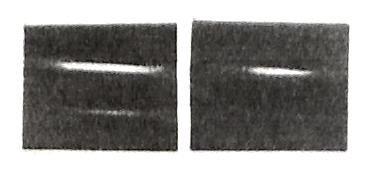
\includegraphics[scale=.97]{eps/12a.eps} &\\[-3pt]
{\fontsize{10pt}{12pt}\selectfont Fig.~1}\relax\qquad\qquad\quad {\fontsize{10pt}{12pt}\selectfont Fig.~2} &\\[7pt]
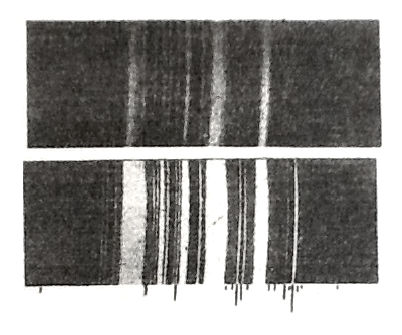
\includegraphics[scale=.97]{eps/12b.eps} & \raisebox{2.5cm}{\begin{tabular}{l}
                                             {\fontsize{10pt}{12pt}\selectfont Fig.~3(1)}\\[1.6cm]
                                             {\fontsize{10pt}{12pt}\selectfont Fig.~3(2)}
                                           \end{tabular}}\\
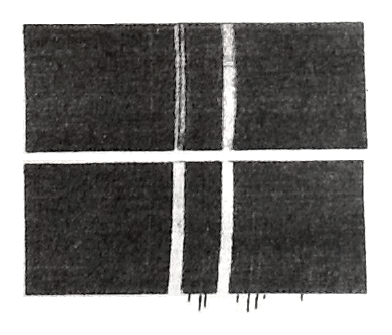
\includegraphics[scale=.97]{eps/12c.eps} & \raisebox{2.5cm}{\begin{tabular}{l}
                                             {\fontsize{10pt}{12pt}\selectfont Fig.~4(1)}\\[2cm]
                                             {\fontsize{10pt}{12pt}\selectfont Fig.~4(2)}
                                           \end{tabular}}\\
\end{tabular}
\end{center}
\vskip -.4cm
{\fontsize{10pt}{12pt}\selectfont {\em Polarisation of Scattering, Fig.~1.~Unmodified; Fig.~2.~\hbox{Modified;} Fig.~3(1).~Incident Spectrum; Fig.~3(2).~Scattered Spectrum; Fig.~4(1). \hbox{Incident} Spectrum; Fig.~4(2).~Scattered Spectrum.}}

\medskip
{\fontsize{10pt}{12pt}\selectfont {\em The first Raman spectra demonstrating the line nature of the Raman scattered radiation (see pages \pageref{pageref-1} and \pageref{pageref-2} for explanation).}}\relax
\end{figure}

\vfill\eject


\noindent
{\em Nature of the new radiation}
\medskip

The discovery set out above naturally opens up an array of problems for investigation. The most pressing question is, How is the modified scattered radiation, as we may call it, generated by the molecules of the liquid? As a tentative explanation, we may adopt the language of the quantum theory, and say that the incident quantum of radiation is partially absorbed by the molecule, and that the unabsorbed part is scattered. The suggestion does not seem to be altogether absurd and indeed such a possibility is already contemplated in the Kramers-Heisenberg theory of dispersion. If we accept the idea indicated above, then the difference between the incident and scattered quanta would correspond to a quantum of absorption by the molecule. The measurement of the frequencies of the new spectral lines thus opens a new pathway of research into molecular spectra, particularly those in the infra-red region.

If a molecule can take up part of the incident quantum of radiation and scatter the remaining part, then it might also be capable of adding a quantum of its own characteristic frequency to the incident-radiation when scattering it. In such a case we should expect a modified line of {\em increased} frequency. Such a result appears to be shown in Fig. 3(2) of Plate XII, as a solitary line in the extreme left of the photograph. This result, however, requires to be confirmed by more photographs and with other liquids. So far it would appear that a degradation of frequency is more probable than an enhancement. It is too early to speculate at present on the origin of the continuous radiation observed in some cases, whether it is due to changes in the molecule itself, or whether it arises from inelastic collisions of the second kind within the liquid, resulting in {\em partial} transformation of the incident quantum of radiation into translatory kinetic energy of the molecules. When further data are obtained, it should be possible to express a definite opinion of this point, and also on the role played by the solvent in the explanation of ordinary fluorescence.

\newpage

\noindent
{\em Relation to thermodynamics}
\vskip .1cm

As explained in the introduction, the ordinary scattering of light can be regarded equally well as a molecular effect and as a bulk effect arising from the thermodynamic fluctuations of the whole me\-dium. The question arises whether the new type of secondary radiation is exclusively a molecular effect or not, and whether it is related in any way to thermodynamics. The question is obviously one to be answered by experiment and theory conjointly. The comparative study of the effect at different temperatures and in different states of aggregation of matter is obviously of great importance in this connection. It has already been remarked that the effect is observable in gases and vapours and indeed it is found possible to determine its intensity and polarisation in the gaseous state. It is also of great interest to remark that the solid crystal ice also shows the sharp modified lines in the scattered-spectrum in approximately the same positions as pure water. The only observations made with amorphous solids are with optical glass. Here the modified scattered-spectrum consists of diffuse bands and not sharp lines. Whether this is generally true for all amorphous solids, and whether any changes occur at low and high temperatures remains to be determined by experiment.

\medskip
\noindent
{\em Coherent or non-coherent radiation?}
\smallskip

An important question to be decided in the first instance by experiment is whether the modified scattered-radiations from the different molecules are incoherent with each other. One is tempted to assume that this must be the case, but a somewhat astonishing observation made with liquid carbon dioxide contained in steel observation vessels gives us pause here. It was found on blowing off the CO$_{2}$ by opening a stop-cock, a cloud formed within the vessels which scattered light strongly in the ordinary way. On viewing the cloud through the complementary filter, the scattered-radiation of modified frequency also brightened up greatly. This would suggest that the assumption of non-coherence is unjustifiable. Further, some qualitative observations suggest that the modified scattering by a mixture of carbon disulphide and methyl alcohol also brightens up notably at the critical solution temperature. Quantitative observations are necessary to decide the very fundamental question here raised.

\medskip
\noindent
{\em Possible $X$-Ray analogies}
\vskip .1cm

\index{Raman, Chandrasekhara Venkata!Papers/Publications/Addresses}

If a quantum of radiation can be absorbed in part and scattered in part in the optical region of the spectrum, should not similar phenomena also occur in X-ray-scattering? The type of scattering discovered by Prof.\@ Compton\index{Compton, A.H.} may possibly be only one of numerous other types of scattering with modified frequencies, some with a line-spectrum and some in the nature of continuous radiation. The extreme ultra-violet region of the spectrum may also furnish us with numerous examples of the new type of radiation, which clearly occupies a position intermediate between scattering the fluorescence.

\medskip
\noindent
{\em Conclusion}
\vskip .1cm

We are obviously only at the fringe of a fascinating new region of experimental research which promises to throw light on diverse problems relating to radiation and wave-theory. X-ray optics, atomic and molecular spectra, fluorescence and scattering, thermodynamics and chemistry. It all remains to be worked out.

I have to add in conclusion that I owe much to the valuable co-operation in this research of Mr. K.S. Krishnan,\index{Krishnan, K.S.} and the assistance of Mr. S. Venkateswaran\index{Venkateswaran, S.} and other workers in my laboratory.

The line-spectrum of the new radiation was first seen on February 28, 1928. The observation was given publicity the following day.

\bigskip
\heading{Davisson on Raman}
\addtocontents{toc}{\protect\contentsline{section}{Davisson on Raman}{\thepage}}
\index{Davisson, C.J.|(}
\smallskip

\lhead[{\it\fontsize{9pt}{9pt}\selectfont\thepage}]{\it{\fontsize{9pt}{11pt}\selectfont Davisson on Raman}}

\noindent
An unusually candid account of Raman's discovery was written by C.J.\@ Davisson of Bell Laboratories in 1931. It appeared in the {\em Bell Laboratories Record}\index{Bell Laboratories Record@\textit{Bell Laboratories Record}} just after Raman was honoured by the award of the Nobel Prize for Physics in 1930. Five years later, Davisson himself shared a Nobel Prize in Physics with G.P. Thomson\index{Thomson, G.P.} for demonstrating the wave nature of electrons. Very brief extracts from this are quoted in the beginning of this Memoir. I reproduce here the full account:

\eject

\begin{quote}
{\fontsize{10pt}{11.85pt}\selectfont
``In awarding the Nobel Prize in Physics for 1930 to Sir C. V. Raman, the Swedish Academy concurred with physicists the world over in appraising the discovery of the ``Raman Effect'' as one of the most important achievements in physics in recent years.

As on some previous occasions, the award this time is made, nominally at any rate, for a single experimental result of striking importance. Again as on previous occasions, the particular experiment to receive this signal recognition is a rather simple one --- one which might have been made with equipment at hand in almost any physical laboratory in the world at any time during the last forty or fifty years. Indeed, within a year of Raman's announcement of his discovery, the effect was verified and studied by more than forty investigators in countries other than India.

In its simplest form the experiment consists in irradiating a transparent substance with monochromatic light, and observing the spectrum of the light which the substance scatters. Raman found that the scattered-light comprises, in addition to a line of the same wavelength as the incident radiation, a few much fainter lines as well, which additional lines are in a sense satellites of the primary line, moving with it as a group through the spectrum when the wavelength of the primary radiation is altered.

In the first definitive experiment of this kind, Raman photogra\-phed the spectra of the radiation scattered by various organic compounds when illuminated by a part of the spectrum of a mercury arc. On long exposure the plates revealed these additional or secondary lines not present in the primary light. It was found possible to classify these secondary lines into groups each associated with a single one of the primary lines; corresponding members of the various groups are displaced in frequency each by the same amount from its primary. The different groups may overlap in the spectrum, making the sorting out difficult but not impossible. A group may extend on both sides of the primary; as a rule, more and stronger lines are found on the side of lower frequencies. Such lines as do appear on the high frequency side are found always to be matched by lines of equal displacement on the low frequency side. It is as if the scattering material has at its disposal a small collection of frequencies which it can add to that of the incident-light or subtract from it, and as if it prefers subtraction to addition. These simple numerical relationships distinguish the \hbox{Raman} Effect from the somewhat similar phenomenon of fluorescence --- these and the fact that the Raman Effect appears to be a universal phenomenon observable with any transparent medium, gaseous, liquid or solid, whereas fluorescence is exhibited by a limited class of materials only.


The simple numerical relationships which have been mentioned as characteristic of the Raman Effect, and one other which is to be described further on, are easily explained in terms of light quanta and the known properties of molecules. This is one of the reasons for regarding the discovery of the Raman Effect as an event of great importance; it makes an addition to the list of phenomena which are conveniently interpreted by regarding light as a corpuscular as well as a wave phenomenon.


Since Einstein\index{Einstein, Albert} in 1906 rehabilitated the corpuscular theory of light to explain the photoelectric effect, and more especially since the discovery of the Compton effect\index{Compton Effect} in 1924, it has become steadily more imperative to recognise that light has these two apparently irreconcilable aspects; a beam of light is a flight of particles or a propagation of trains of waves, depending upon the particular phenomenon which is to be explained or visualised. In explaining some phenomena it is even necessary, or at least convenient, to oscillate between the two views at different stages of the argument. In such cases, translation from one to the other is made by means of two well-established laws: the energy of the light particles or photons is strictly proportional to the frequency (waves per second) of the associated undulations, and similarly the momentum of the photons is strictly proportional to the wave number (waves per centimetre) of the undulations. The factor of proportionality is in both cases the so-called Planck constant $h$.


In the corpuscular explanation, the Raman Effect is due to interchanges of energy occurring in encounters between photons of the incident light and molecules of the scattering material. Photons emerge from these encounters with altered energy; they constitute the scattered-light of altered frequency and altered wavelength which Raman detected. Now every kind of molecule or atom has the following peculiar property; its internal energy is limited to certain definite discrete values. The molecule is capable of existence only at certain `energy levels', and can accept or give up energy only in amounts which will raise or lower it, from the particular level in which it happens to be to another of its levels.

Thus the photons may give up to the molecules only one or another of these characteristic amounts of energy, and, in
consequence of the direct proportionality between energy and frequency, the frequency of the associated waves should be lowered only by corresponding amounts. It is for this reason that the Raman spectrum is a spectrum of sharp lines. The frequency displacements in the Raman spectrum should correspond to differences between energy levels of the molecules; and in cases in which these latter are already known, this relationship is verified.

The Raman lines on the high frequency side of the primary line may be explained on the general principle that processes of the kind mentioned in the last paragraph are necessarily reversible. If it is possible for a photon to give up a part of its energy in raising a molecule from one level to another. it must be possible also for the molecule in passing in the opposite direction to impart an equal amount of energy to a colliding photon. This process is the analogue of what is known in encounters between electrons and atoms as a `collision of the second kind'. The presence of high-frequency components in the Raman spectrum symmetrical with the low-frequency components is due to such encounters. These components are weaker than their companions because at ordinary temperatures nearly all of the molecules are in their state of lowest energy and are incapable therefore of imparting energy.

Thus, the importance of Raman's discovery is due partly to its revealing a previously unknown process in nature, partly to the additional basis of reality which it affords to the photon, and partly to its supplying a new and convenient method of investigating the energy level of molecules.

It was remarked earlier on that the Raman experiment is a rather simple one which might have been made with equipment available in any physical laboratory at any time in recent decades. It was no accident, however, that this particular discovery was made by Raman rather than by someone else. Important discoveries in physics, even quite simple ones, are usually made only by investigators who have cultivated intensively the particular field concerned, and this is strikingly true in the present instance. No one else in recent years has been as assiduous in the study of the scattering of light as Professor \hbox{Raman}. True, in the years just following his graduation from Presidency College,\index{Presidency College} Madras, in 1907, his interest --- if we may judge from\break his publications --- centred chiefly in the vibrations of mechanical systems --- stringed musical instruments in particular --- and other acoustical problems. But even in these years problems in optics claimed a part of his attention. About 1920, however --- three years after he became Sir Taraknath Palit Professor of Physics at Calcutta University --- he turned abruptly from studies in acoustics and devoted himself almost exclusively to optics and particularly to investigations of scattering, both theoretical and experimental. Of one hundred papers and notes published by Raman independently, or in collaboration with his associates and students, since that time, eighty-three deal with problems in optics and forty-nine of these with the scattering of light.

It speaks well for the development of Science in India that Professor Raman apparently owes little or nothing of his
 eminence to direct contact with physicists in other countries. His formal training was received entirely in India, and, except for a single year, he has worked only in his native land. In 1924 he attended the Toronto meeting of the British Association and afterwards carried on his researches for some months at California Institute of Technology.}\relax

{\fontsize{10pt}{11.85pt}\selectfont His previous honours,\index{Raman, Chandrasekhara Venkata!Awards/Distinctions} which have been numerous, include the general presidency of the Indian Science Congress and fellowship in the Royal Society. Knighthood was conferred upon him by King George in 1929. India may well be proud of Sir Chandrasekhara Venkata \hbox{Raman}, her first Nobel Laureate in Science.''}\relax\index{Davisson, C.J.|)}
\end{quote}





